\chapter{Datos y universo de inversión}
\label{chap:datos}

El universo se reconstruye históricamente a partir de la pertenencia al S\&P 500. Una empresa sólo
es elegible cuando pertenecía al índice en ese snapshot; por tanto, no se usa la composición actual
para describir el pasado. Los precios proceden de Yahoo Finance, los fundamentales de Finnhub y las
fechas de publicación de SEC EDGAR. SPY es el benchmark y se excluye explícitamente de las
posiciones.

La cobertura se mide, no se presume. El pipeline identifica reutilizaciones de ticker, como CPQ y
MOB, y evita asociar precios de una empresa posterior a un miembro histórico. La fracción utilizable
es al menos 99,4\% en los años representados, aunque persiste un riesgo residual de supervivencia y
de restatements históricos que se discute en el Capítulo~\ref{chap:limitaciones}.

\begin{figure}[H]
\centering
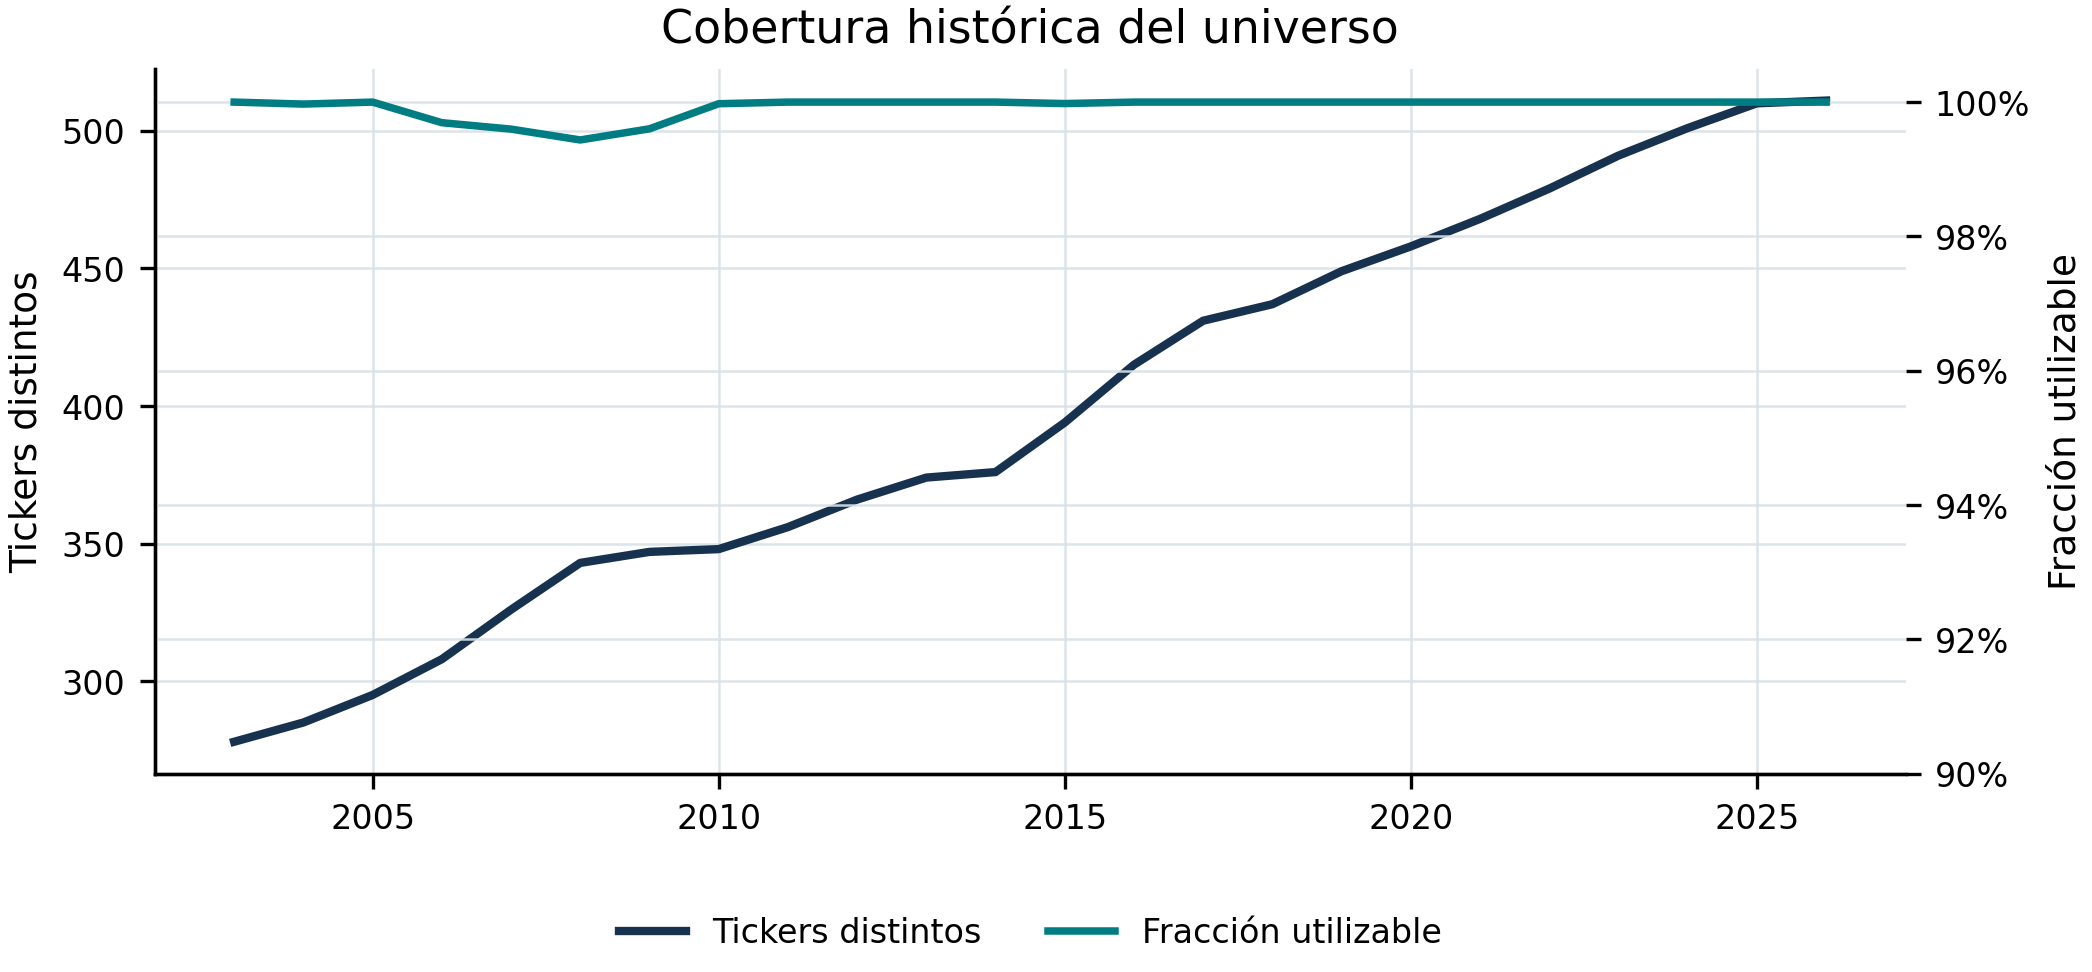
\includegraphics[width=0.93\textwidth]{assets/f03_cobertura.png}
\caption{Cobertura anual del universo histórico. Fuente: \texttt{attribution.json} →
\texttt{universe\_coverage}.}
\end{figure}

El dataset preparado está identificado por el hash
\texttt{b9134b218e3bf7fc156372d61e02056ecfa6036777e0fe84a69df0a92653fbd3}. Guardar la identidad,
y no una copia del dataset dentro de resultados, permite rastrear la procedencia de toda cifra y
evita reutilizar por error una evaluación sobre datos distintos.

\section{Fuentes y función de cada fuente}

Ninguna fuente aislada proporciona todos los elementos necesarios para una evaluación temporalmente
honesta. Yahoo Finance aporta series de precios ajustados que permiten valorar posiciones y calcular
retornos. Finnhub aporta ratios y series fundamentales con los que se construyen las variables de
calidad, valor, crecimiento y parte del riesgo. SEC EDGAR proporciona la fecha de filing de los
10-K y 10-Q; esta fecha establece cuándo el mercado pudo conocer un estado financiero. Por último,
el historial de composición del índice determina qué empresas forman parte del universo invertible
en cada instante.

Esta combinación introduce una jerarquía de confianza. Los precios se usan con la última cotización
disponible antes del snapshot. Los fundamentales no se usan sólo por existir en la descarga: deben
estar asociados a un periodo y a un filing elegible. Los perfiles de Finnhub, como el sector, nunca
entran como señal predictiva; sólo se pueden usar para agrupaciones auxiliares cuando la
configuración solicita neutralización. Esta restricción reduce el riesgo de que una columna moderna
de perfil introduzca información retrospectiva.

La falta de un dato no se interpreta como un retorno nulo ni se sustituye con una media global que
mezcle fechas futuras. El pipeline aplica una imputación basada en la mediana del conjunto de
entrenamiento disponible e incorpora indicadores de ausencia. De esta manera el modelo puede
aprender que la falta de cobertura es informativa, pero no recibe una estimación calculada con el
futuro. Una observación sin precio suficiente o sin fundamental elegible puede quedar fuera de la
cohorte; esa exclusión se registra en la cobertura anual.

\section{Universo dinámico y pertenencia histórica}

El universo no es la lista actual del S\&P 500. Para cada fecha se consulta qué tickers pertenecían
al índice en ese momento y se construye la sección transversal sólo con ellos. Esta decisión evita
un sesgo frecuente: usar empresas que sobrevivieron y permanecen hoy en el índice para evaluar
periodos en los que otras empresas ya habían sido expulsadas, adquiridas o quebrado. La literatura
ha documentado que esta selección puede inflar de forma material las conclusiones de rendimiento
(Brown et al., 1992).

La corrección no equivale a eliminar todo sesgo de supervivencia. Las fuentes gratuitas pueden no
ofrecer la misma profundidad para firmas retiradas, algunos fundamentales históricos se han
restatado y la disponibilidad puede variar por año. La diferencia es metodológica: el trabajo mide
esa cobertura, expone sus huecos y evita tratarlos como si no existieran. La Figura de cobertura
mostrada antes hace visible tanto el crecimiento del número de tickers como la fracción de filas que
realmente pueden usar el pipeline.

Un caso adicional es la reutilización de símbolos. Un ticker puede corresponder a una empresa
histórica y, años después, a otra distinta. CPQ dejó de pertenecer al índice en 2002, pero una serie
de precios descargada posteriormente no necesariamente representa a Compaq; MOB presenta un caso
análogo. Si se unieran esas series por ticker sin comprobar el intervalo de pertenencia, se crearía
una historia de precios inexistente. La guarda de reciclaje compara la primera fecha de precio con
el intervalo de membresía y excluye los símbolos incompatibles.

\section{Identidad, materialización y trazabilidad}

El dataset se materializa una vez bajo una identidad que resume fuentes, rango temporal, universo,
cadencia, horizonte, lag y versiones de transformación. Si dos evaluaciones resuelven la misma
identidad, pueden reutilizar la materialización; si cualquiera de esos elementos cambia, se crea un
dataset distinto. Los resultados no contienen una copia del panel: conservan la referencia y su
hash. Esta elección reduce duplicación y permite reconstruir de qué datos procedió un resultado.

La identidad de evaluación incluye además el hash del dataset. Sin esa condición, dos estudios con
parámetros nominalmente iguales pero datos distintos podrían compartir por error una clave de caché.
Por tanto, la trazabilidad no es un detalle administrativo: impide que una métrica calculada sobre
un panel se atribuya a otro. En los anexos se conserva el hash de dataset, la clave de evaluación,
el identificador del estudio y las rutas de los artefactos que alimentan cada tabla y figura.

\section{Ventanas temporales del experimento}

El modelo necesita historia anterior para entrenarse. Con una ventana móvil de ocho años y primer
snapshot de la evaluación en 2015, la información de entrenamiento procede de periodos anteriores,
siempre que sus etiquetas ya hayan cerrado. La ventana de selección se extiende de 2015 a 2024 y
contiene 117 cohortes mensuales. Los datos de 2025--2026 se separan como era reservada antes de
elegir variables, pesos o reglas de cartera. Así, observar un buen resultado reservado no permite
volver atrás para retocar el ganador.

Esta separación no convierte automáticamente 2025--2026 en una prueba definitiva. El horizonte de
doce meses deja varias etiquetas abiertas y reduce la información independiente. Su función es más
exigente que una fila adicional en la tabla de selección: es una comprobación externa del modelo ya
congelado, cuya interpretación se mantiene deliberadamente prudente en el Capítulo~\ref{chap:resultados}.

La Tabla~\ref{tab:cobertura-anual} documenta la cobertura año a año desde 2003, es decir, incluyendo
los años que sólo se usan como historia de entrenamiento y nunca como cohortes de evaluación.

\begin{longtable}{lrrrrr}
\caption{Cobertura anual del universo y calidad del panel. «Cobertura» es la fracción de los miembros reales del índice que llega al panel; «fracción utilizable» mide la calidad dentro de él y no dice nada sobre los que faltan.}\label{tab:cobertura-anual}\\
\toprule
Año & Miembros S\&P 500 & Tickers del panel & Cobertura & Filas utilizables & Fracción utilizable \\
\midrule
\endfirsthead
\toprule
Año & Miembros S\&P 500 & Tickers del panel & Cobertura & Filas utilizables & Fracción utilizable \\
\midrule
\endhead
\midrule
\multicolumn{6}{r}{\footnotesize Continúa en la página siguiente}\\
\endfoot
\bottomrule
\endlastfoot
2003 & 494 & 277 & 56,1\% & 2.752 & 100,00\% \\
2004 & 495 & 284 & 57,4\% & 3.369 & 99,97\% \\
2005 & 497 & 294 & 59,2\% & 3.430 & 100,00\% \\
2006 & 497 & 307 & 61,8\% & 3.565 & 99,69\% \\
2007 & 497 & 325 & 65,4\% & 3.702 & 99,60\% \\
2008 & 498 & 342 & 68,7\% & 3.869 & 99,43\% \\
2009 & 499 & 346 & 69,3\% & 3.994 & 99,60\% \\
2010 & 497 & 347 & 69,8\% & 4.101 & 99,98\% \\
2011 & 497 & 355 & 71,4\% & 4.140 & 100,00\% \\
2012 & 497 & 365 & 73,4\% & 4.254 & 100,00\% \\
2013 & 497 & 373 & 75,1\% & 4.365 & 100,00\% \\
2014 & 499 & 375 & 75,2\% & 4.419 & 100,00\% \\
2015 & 502 & 392 & 78,1\% & 4.564 & 99,98\% \\
2016 & 506 & 413 & 81,6\% & 4.800 & 100,00\% \\
2017 & 505 & 429 & 85,0\% & 4.971 & 100,00\% \\
2018 & 505 & 435 & 86,1\% & 5.050 & 100,00\% \\
2019 & 505 & 448 & 88,7\% & 5.148 & 100,00\% \\
2020 & 505 & 457 & 90,5\% & 5.335 & 100,00\% \\
2021 & 505 & 467 & 92,5\% & 5.448 & 100,00\% \\
2022 & 503 & 479 & 95,2\% & 5.594 & 100,00\% \\
2023 & 503 & 491 & 97,6\% & 5.738 & 100,00\% \\
2024 & 503 & 501 & 99,6\% & 5.828 & 100,00\% \\
2025 & 503 & 510 & 101,4\% & 5.905 & 100,00\% \\
2026 & 503 & 510 & 101,4\% & 2.998 & 100,00\% \\
\end{longtable}


Dos observaciones sobre esa tabla. La primera es que el número de \textit{tickers} distintos crece
de 278 en 2003 a más de 500 en los años recientes, lo que refleja que la reconstrucción de la
pertenencia histórica es más completa cuanto más cerca está del presente: es una limitación de la
fuente, no una propiedad del índice, que ha tenido alrededor de quinientos componentes durante todo
el periodo. La segunda es que la fracción de filas utilizables se mantiene muy próxima a uno en
todos los años. Esto último debe leerse con cuidado: mide qué proporción de las filas efectivamente
construidas supera los controles de calidad, no qué proporción de las empresas que existieron
llegaron a construirse. El sesgo de supervivencia que preocupa no se manifiesta como filas
defectuosas sino como empresas ausentes, y esa ausencia no es observable desde el propio panel.

\section{El catálogo de variables y su reparto entre agentes}

Las variables que alimentan a los agentes no se eligen a mano ni por conveniencia. El catálogo
declara bloques temáticos, cada bloque se asigna a un agente, y el conjunto de variables que entra
en el estudio es una decisión del propio protocolo. La Tabla~\ref{tab:features-bloque} resume esos
bloques con sus diagnósticos.

\begin{table}[H]
  \centering
  \small
  \caption{Bloques de variables, agente asignado y diagnósticos univariantes.}
  \label{tab:features-bloque}
  \begin{tabular}{llrrrr}
\toprule
Bloque & Agentes & Vars. & Cobertura & Rank-IC univ. & Importancia \\
\midrule
market liquidity & risk & 4 & 99,9\% & 0,0177 & 107,3 \\
quality core & quality & 9 & 86,6\% & 0,0133 & 42,3 \\
value cashflow & value & 2 & 81,9\% & 0,0126 & 34,2 \\
value core & value & 7 & 83,4\% & 0,0080 & 105,7 \\
quality efficiency & quality & 6 & 82,7\% & 0,0047 & 72,6 \\
fundamental stability & growth & 5 & 88,1\% & 0,0044 & 106,1 \\
momentum trend & momentum & 4 & 99,9\% & 0,0039 & 120,1 \\
financial strength & quality & 9 & 89,5\% & 0,0031 & 44,8 \\
growth acceleration & growth & 8 & 90,1\% & 0,0013 & 117,1 \\
price risk & risk & 8 & 99,8\% & -0,0016 & 85,3 \\
momentum core & momentum & 6 & 99,6\% & -0,0036 & 130,3 \\
(no declarado) & — & 7 & 92,3\% & -0,0055 & 71,2 \\
\bottomrule
\end{tabular}

  \caption*{Fuente: \artefacto{evidence/feature\_catalog.json} y
  \artefacto{evidence/feature\_diagnostics.parquet}. El Rank-IC univariante es el de cada variable
  por separado, sin modelo; la importancia es la media asignada por LightGBM.}
\end{table}

\begin{figure}[H]
  \centering
  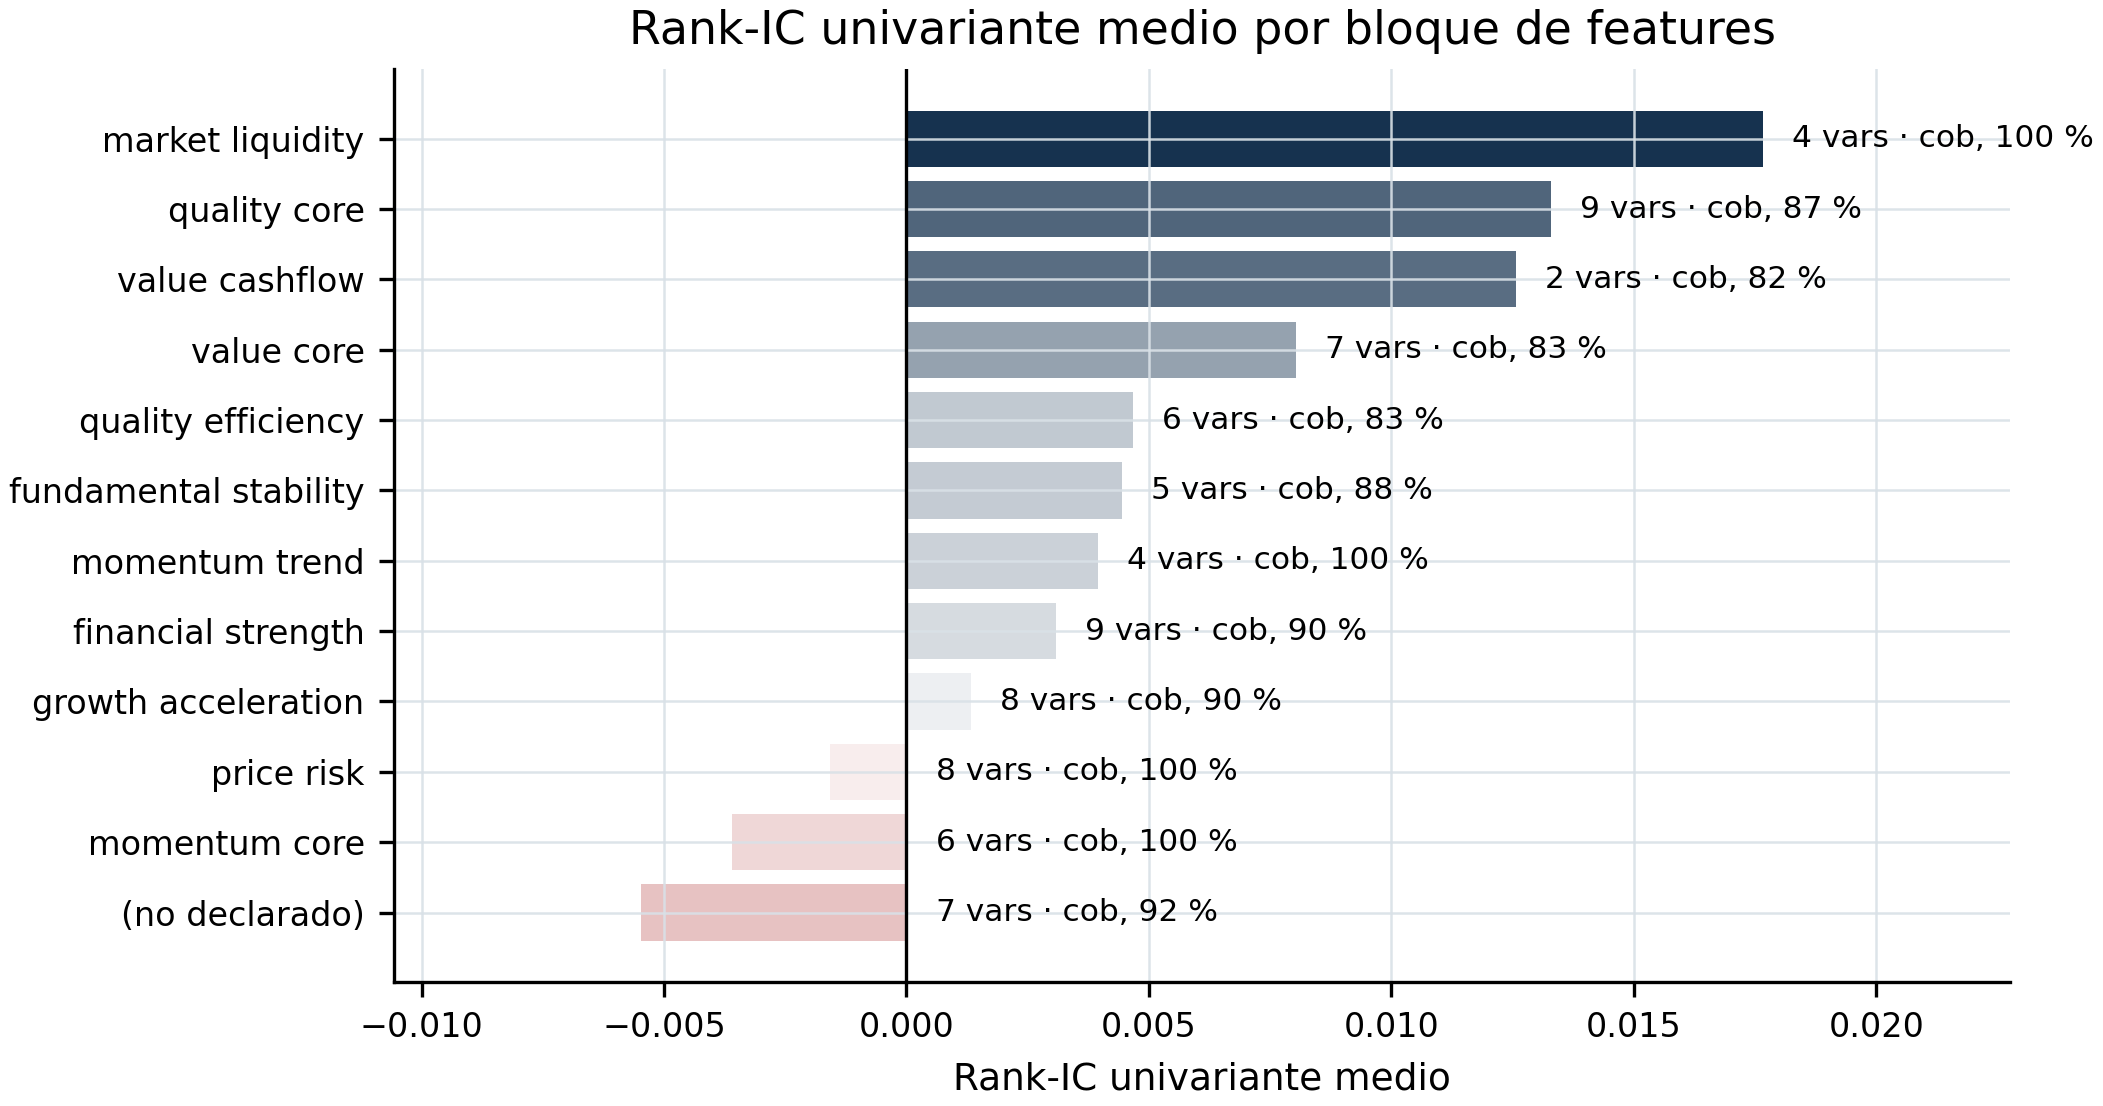
\includegraphics[width=0.94\textwidth]{assets/f03_features_bloques.png}
  \caption{Rank-IC univariante medio por bloque. Fuente:
  \artefacto{evidence/feature\_diagnostics.parquet}.}
  \label{fig:features-bloques}
\end{figure}

La tabla exige tres advertencias metodológicas, y las tres importan para no sobreinterpretarla.

La primera es que las dos fuentes no coinciden exactamente. El catálogo declara 68 variables con su
bloque y su agente; el fichero de diagnósticos contiene 73 filas, porque incluye siete columnas
derivadas que el catálogo no declara por separado --- componentes descompuestos de otras variables
--- y omite dos que sí declara pero para las que no llegó a calcular diagnósticos. La tabla hace una
unión de ambas y agrupa esas siete bajo la etiqueta «no declarado» en lugar de descartarlas
silenciosamente. Es una asimetría menor, pero ocultarla habría significado presentar un recuento que
no coincide con ninguno de los dos artefactos.

La segunda es que el estado de selección vale \texttt{candidate} en las 73 filas. El artefacto no
registra
qué variables fueron efectivamente podadas por el mecanismo de estabilidad fuera de muestra, de modo
que \emph{esta tabla no puede leerse como «variables seleccionadas frente a descartadas»}. Describe
el catálogo declarado y sus diagnósticos, nada más.

La tercera es sobre la magnitud de las cifras. Los Rank-IC univariantes son diminutos --- el mayor
bloque apenas alcanza 0,0177 --- frente al 0,1090 del sistema completo. No es una contradicción: es
exactamente el argumento a favor de combinar. Ninguna variable aislada ordena el mercado, y la
capacidad predictiva aparece al combinar muchas señales débiles mediante modelos no lineales y una
ponderación aprendida. La Tabla~\ref{tab:features-top} muestra los extremos de esa distribución.

\begin{table}[H]
  \centering
  \small
  \caption{Variables con mayor y menor Rank-IC univariante.}
  \label{tab:features-top}
  \begin{tabular}{lllrr}
\toprule
Feature & Bloque & Agentes & Cobertura & Rank-IC univ. \\
\midrule
factor\_gap\_21d & market liquidity & risk & 99,9\% & 0,0540 \\
factor\_cash\_conversion & fundamental stability & growth & 82,7\% & 0,0370 \\
factor\_asset\_turnover & quality efficiency & quality & 88,8\% & 0,0353 \\
factor\_rotc & quality core & quality & 86,6\% & 0,0338 \\
factor\_range\_63d & price risk & risk & 99,9\% & 0,0297 \\
factor\_roic & quality core & quality & 90,9\% & 0,0293 \\
factor\_roe & quality core & quality & 90,9\% & 0,0281 \\
factor\_range\_21d & price risk & risk & 99,9\% & 0,0278 \\
factor\_ev\_revenue & value core & value & 88,7\% & 0,0259 \\
factor\_mom\_volatility & momentum trend & momentum & 99,8\% & 0,0241 \\
factor\_ps & value core & value & 88,8\% & 0,0236 \\
factor\_roa & quality core & quality & 94,4\% & 0,0223 \\
factor\_roic\_trend & fundamental stability & growth & 89,4\% & -0,0145 \\
factor\_receivables\_turnover & quality efficiency & quality & 79,3\% & -0,0147 \\
factor\_roe\_stability & fundamental stability & growth & 90,0\% & -0,0147 \\
factor\_pb & value core & value & 90,8\% & -0,0236 \\
factor\_beta\_252d & price risk & risk & 99,8\% & -0,0375 \\
\bottomrule
\end{tabular}

  \caption*{Fuente: \artefacto{evidence/feature\_diagnostics.parquet}. Doce primeras y cinco últimas
  de las 73 disponibles, ordenadas por Rank-IC univariante.}
\end{table}

Obsérvese que el bloque de liquidez de mercado, asignado al agente \textit{risk}, encabeza la
clasificación por bloques, mientras que los bloques de \textit{momentum} aparecen en la parte baja e
incluso con signo negativo. Es coherente con lo que el Capítulo~\ref{chap:agentes} documenta sobre
el dominio de \textit{risk} y la debilidad de \textit{momentum}, y sugiere que esa jerarquía ya está
presente en los datos antes de cualquier modelo.
